\section{Ipoteza de Broglie. Difracția electronilor. Aplicații}

Analog cu dualismul undă-corpuscul în cazul undelor electromagnetice, Louis de Broglie asociază oricărei microparticule în mișcare cu energia $E$ și impulsul $p$ o undă caracterizată prin frecvența $\nu$ și lungimea de undă $\lambda$, cu relațiile dintre mărimi
\[
    E = h \nu
    \begin{Bmatrix}
        \nu & \lambda \\
        E   & p
    \end{Bmatrix}
    p = \frac{h}{\lambda}
\]

De Broglie a presupus că lungimea de undă a undelor asociate microparticulelor
trebuie să fie dată tot de relația \( \lambda = \frac{h}{p} \), unde $p$ este
impulsul microparticulei.

\parbreak

Ipoteza de Broglie afirmă că oricărei microparticule care posedă un impuls $p$
i se poate asocia în mod formal o undă cu lungimea de undă
\( \lambda_B = \frac{h}{p} \), numită lungime de undă de Broglie.

Undelor electromagnetice le sunt asociați fotonii, care nu au masă de repaus.
Analog, undele de Broglie sunt asociate particulelor cu masă de repaus:
electroni, protoni, neutroni, particule \alpha, molecule de hidrogen. În
concluzie, radiația electromagnetică are proprietăți ondulatorii și
corpusculare, asemenea radiației corpusculare.

\subsection*{Experimentul Davisson-Germer}

Fizicienii Davisson și Germer au confirmat experimental ipoteza de Broglie,
demonstrând că electronii în mișcare prezintă proprietăți ondulatorii, prin
generarea fenomenelor de difracție însoțite de interferență.

\begin{wrapfigure}{r}{0.45\textwidth}
    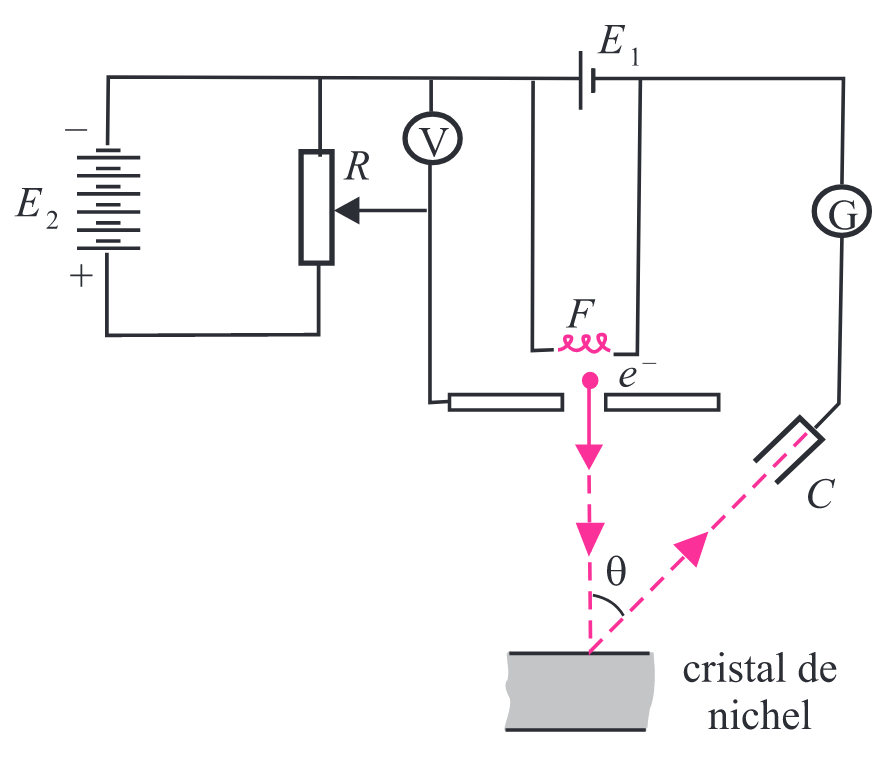
\includegraphics[width=0.45\textwidth]{fig/davisson_germer}
    \caption{Schema experimentului}
\end{wrapfigure}

Filamentul $F$, alimentat de sursa $E_1$, emite electroni care sunt accelerați
într-un tun electronic, alimentat de sursa $E_2$. Tensiunea de accelerare $U$
este controlată de reostatul $R$ și măsurată cu voltmetrul $V$.

Fasciculul monoenergetic de electroni, numit \emph{monocromatic}, care iese din
tunul electronic, are energia:
\begin{equation}
    \frac{m_e v^2}{2} = eU \label{eq:1}
\end{equation}

Fasciculul cade pe un monocristal de nichel, iar fasciculul difractat este
captat de un cilindru Faraday $C$ colector. Curentul de electroni este măsurat
de galvanometrul $G$.

Se observă că intensitatea fasciculului de electroni difractați prezintă maxime
și minime în funcție de $U$ și unghiul de incidență $\theta$.

Din relația \eqref{eq:1} rezultă \( v = \sqrt{\frac{2eU}{m_e}} \).

În cazul nerelativist avem impulsul \( p = m_e v = \sqrt{2em_e U} \), iar
lungimea de undă de Broglie asociată este:
\[
    \lambda_B = \frac{h}{p} = \frac{h}{\sqrt{2em_e} U}
    = \frac{h}{\sqrt{2em_e}} \cdot \frac{1}{\sqrt{U}}
    = \frac{12,23 \cdot 10^{-10}}{\sqrt{U}}
\]

Pentru un potențial de accelerare \( V = 54 \unit{V} \), lungimea de undă
este de același ordin de mărime cu lungimea de undă a radiației X:
\begin{equation}
    \lambda_B = \frac{12,23 \cdot 10^{-10}}{\sqrt{54}}
    = 1,664 \cdot 10^{-10} \unit{m} \label{eq:2}
\end{equation}

Fenomenele de difracție pot fi observate când unda interacționează cu o „rețea
de difracție” a cărei constantă de rețea are dimensiunile comparabile cu
lungimea de undă (\( 10^{-10} \unit{m} \)).

\begin{wrapfigure}{r}{0.45\textwidth}
    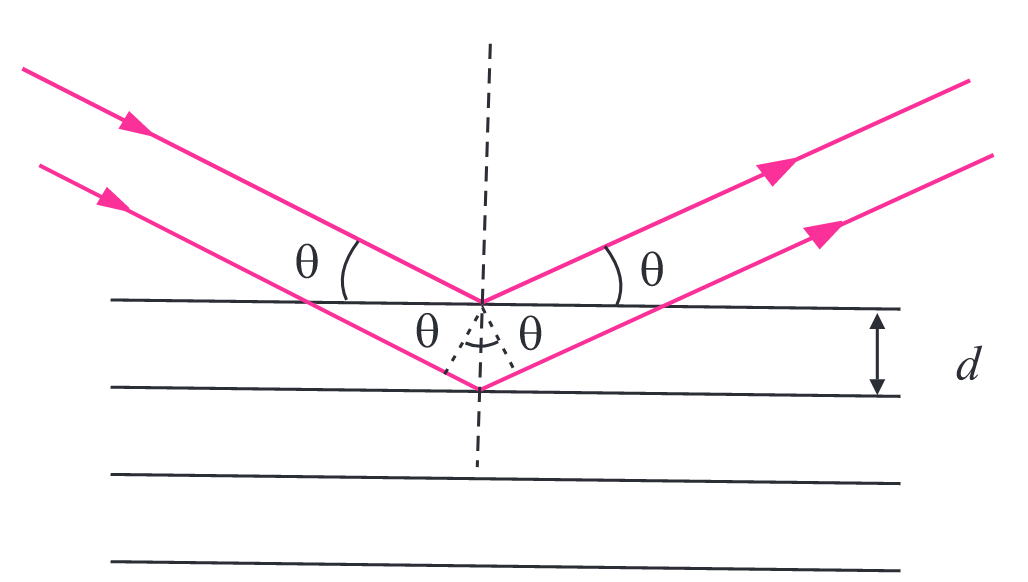
\includegraphics[width=0.45\textwidth]{fig/monocristal}
    \caption{Difracția razelor X pe un monocristal}
\end{wrapfigure}

Atomii monocristalului sunt așezați ordonat, distanța dintre doi atomi vecini
fiind de ordinul \( 10^{-10} \unit{m} \). Această aranjare regulată în nodurile
rețelei cristaline conferă proprietățile unei rețele de difracție
tridimensionale.

În urma studierii difracției razelor X pe monocristale, Bragg a stabilit că
intensitatea fasciculului difractat trece prin valori maxime în cazul:
\begin{equation}
    2d\sin\theta = k\lambda, k \in \mathbb{N^*} \label{eq:3}
\end{equation}
unde:
\begin{itemize}
    \item $\theta$ este unghiul format de planul reticular cu direcția fasciculului incident, respectiv cel difractat.
    \item $d$ este constanta rețelei, adică distanța dintre două plane reticulare.
    \item $\lambda$ este lungimea de undă a radiației.
    \item $2d\sin\theta$ este diferența de drum dintre razele difractate de două plane reticulare vecine.
\end{itemize}

În cazul în care particulele suferă o difracție, se aplică relația
\eqref{eq:3}. Pentru \( d = 0,91 \cdot 10^{-10} \unit{m} \), $k = 1$,
$U = 54 \unit{V}$, tensiune la care se obține primul maxim pentru
$\theta = 65^\circ$, se obține:
\begin{equation}
    \lambda_B = 2d\sin\theta = 2 \cdot 0,91 \cdot 10^{-10} \cdot 0,906 = 1,65 \cdot 10^{-10} \unit{m} \label{eq:4}
\end{equation}

Valorile obținute în relațiile \eqref{eq:2} și \eqref{eq:4} se află în concordanță, confirmând că
electronii în mișcare au proprietăți ondulatorii.

Lungimea de undă de Broglie este invers proporțională cu masa particulelor cărora le este asociată.

Microparticulele, numite \emph{particule cuantice}, sunt radical diferite de
particulele clasice, supunându-se unor legi specifice. Nu sunt nici particule,
nici unde în sens clasic, comportamentul lor reflectând dualismul
corpuscul-undă.

Deși unda de Broglie asociată microparticulelor nu este o undă în sensul clasic
al cuvântului, este folosită această noțiune.

La nivel macroscopic, un corpuscul nu poate avea proprietăți ondulatorii, iar
unda nu poate fi concepută ca un flux de particule discrete. Particulele
cuantice aparțin însă nivelului cuantic, fiind radical diferite de unde și
corpusculi. De exemplu, ele nu au traiectorii.

Asupra sistemelor cuantice putem face doar afirmații statistice.

\subsection*{Microscopul electronic}

Microscopul electronic este o aplicație a ipotezei lui de Broglie. Un
fasciculul de electroni cade pe un preparat și îl traversează, variațiile de
grosime ale preparatului devenind variații de intensitate a fasciculului.
Utilizând câmpuri electrice sau magnetice, traiectoriile electronilor sunt
asemănătoare traiectoriilor razelor de lumină dintr-un microscopic optic.

În cazul microscopului optic, pentru a distinge două puncte, distanța dintre
ele trebuie să fie mai mare decât lungimea de undă a luminii folosite, adică
mai mare decât zecimi de microni (puterea de separare).

În locul lentilelor optice se găsesc bobinele parcurse de curent electric
(\emph{lentile magnetice}) sau electrozii încărcați electric
-- \emph{lentile electrice} -- ce pot focaliza și defocaliza un fascicul de
electroni.

\parbreak

\begin{minipage}{0.6\textwidth}
    \captionsetup{type=figure}
    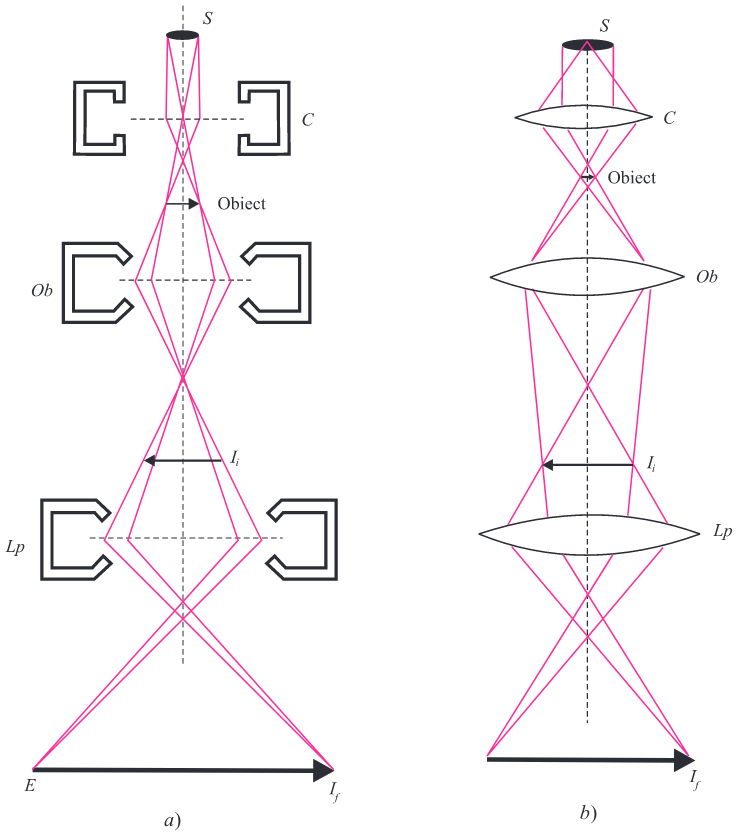
\includegraphics[width=\textwidth]{fig/microscop}
    \caption{Schema microscopului electronic și a microscopului optic}
\end{minipage}%
\hspace{0.5cm}%
\begin{minipage}{0.3\textwidth}
    \begin{itemize}[left=0pt,label=]
        \item $S$ -- sursa de electroni (a) sau lumină (b)
        \item $C$ -- condensator
        \item $Ob$ -- obiectiv
        \item $I_i$ -- imagine intermediară
        \item $Lp$ -- lentilă de proiecție
        \item $I_f$ -- imagine finală
        \item $E$ -- ecran fluorescent
    \end{itemize}
\end{minipage}

\parbreak

Datorită lungimii de undă mult mai mici a undelor asociate electronilor,
puterea de separare a microscopului electronic este mult mai mare decât a
microscopului optic. Transformarea imaginii în una luminoasă se realizează cu
ajutorul unui ecran fluorescent.

Probele examinate trebuie să fie sub formă de pelicule foarte subțiri, din
cauza puterii de pătrundere mici a electronilor.

Au fost construite și microscoape protonice și ionice, care pot mări de 10-15
ori mai mult decât un microscop electronic.
